% qliff — progress deck.
% Plain DEFAULT beamer (no theme/colour overrides), 16:9.
% Lean slides; speaker detail is kept separately.
\documentclass[aspectratio=169]{beamer}

\usepackage{amsmath, amssymb}
\usepackage{booktabs}
\usepackage{graphicx}
\usepackage{tikz}
\usepackage{pgfplots}
\pgfplotsset{compat=1.18}
\usetikzlibrary{positioning, fit, arrows.meta, backgrounds, decorations.pathreplacing}

\newcommand{\code}[1]{\texttt{#1}}

% Credits-slide person card: figs/<name>.{jpg,png} if present, else initials.
% Args: #1 image path, #2 initials, #3 name, #4 affiliation, #5 work.
\newcommand{\person}[5]{%
  \begin{column}{0.24\textwidth}
    \centering
    \IfFileExists{#1}{%
      \includegraphics[width=2.3cm,height=2.3cm,keepaspectratio]{#1}%
    }{%
      \begin{tikzpicture}
        \node[draw, rounded corners, minimum width=2.3cm, minimum height=2.3cm,
              fill=black!8, text=black!55] {\Large\bfseries #2};
      \end{tikzpicture}%
    }\\[3pt]
    \textbf{#3}\\[1pt]
    {\scriptsize #4}\\[2pt]
    {\scriptsize\itshape #5}
  \end{column}%
}

\title{qliff}
\subtitle{A Clifford and noisy stabilizer simulator}
\author{}
\date{}

\begin{document}

\begin{frame}
  \titlepage
  \begin{center}
    \small Stim-class clean speed, and the coherent noise stim cannot touch.
  \end{center}
\end{frame}

% ======================================================================
\section{What this is}
% ======================================================================

\begin{frame}{What is qliff?}
  \begin{itemize}
    \item A \textbf{stabilizer simulator}: simulates a class of quantum circuits without approximation.
    \item It tracks $\sim n^2$ bookkeeping, not $2^n$ amplitudes.
    \item Two jobs: \begin{itemize}
      \item \textbf{clean Clifford} at stim speed, and
      \item \textbf{noisy} simulation including coherent noise stim cannot do.
    \end{itemize}
    \item Ships decoder-ready \textbf{QEC} outputs (detectors, observables, error model).
  \end{itemize}
  \vfill
  \begin{center}
  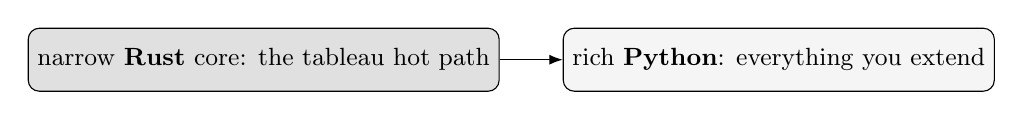
\begin{tikzpicture}[font=\small, node distance=8mm]
    \node[draw, rounded corners, fill=black!12, minimum height=8mm] (rust) {narrow \textbf{Rust} core: the tableau hot path};
    \node[draw, rounded corners, fill=black!4, minimum height=8mm, right=of rust] (py) {rich \textbf{Python}: everything you extend};
    \draw[-{Latex}] (rust) -- (py);
  \end{tikzpicture}
  \end{center}
\end{frame}

\begin{frame}{Built on work from}
  \begin{columns}[T]
    \person{figs/aaronson.jpg}{SA}{Scott Aaronson}{UT Austin}{Quantum complexity, CHP, BosonSampling}
    \person{figs/gottesman.jpg}{DG}{Daniel Gottesman}{Univ.\ of Maryland (QuICS)}{Stabilizer formalism, fault tolerance}
    \person{figs/ng.jpg}{HKN}{Hui Khoon Ng}{NUS (CQT), Singapore}{Approximate QEC}
    \person{figs/gidney.jpg}{CG}{Craig Gidney}{Google Quantum AI}{Stim, Cirq, Sparse Bloom}
  \end{columns}
\end{frame}

\begin{frame}{Why is simulating qubits hard?}
  A qubit is a blend of 0 and 1, so $n$ qubits need $2^n$ numbers to write down in full.
  \vfill
  \begin{center}
  \begin{tikzpicture}
  \begin{semilogyaxis}[
      width=0.8\textwidth, height=0.58\textheight,
      xlabel={qubits $n$}, ylabel={numbers to store},
      ymin=1e2, ymax=1e95, xmin=0, xmax=310,
      ytick={1e3,1e20,1e40,1e60,1e80}, grid=both, major grid style={black!10},
    ]
    \addplot[blue, very thick, mark=*] coordinates {
      (10,1e3) (50,1.1e15) (100,1.3e30) (150,1.4e45) (200,1.6e60) (250,1.8e75) (300,2e90) };
    \addplot[red, dashed, no markers, thick] coordinates {(0,1e80) (310,1e80)};
    \node[red, anchor=south east, font=\scriptsize] at (axis cs:300,1e80) {atoms in the universe};
  \end{semilogyaxis}
  \end{tikzpicture}
  \end{center}
  \vfill
  \begin{center}\small Past $\sim$270 qubits the state has more numbers than the universe has atoms. You need a shortcut.\end{center}
\end{frame}

\begin{frame}{What is a stabilizer?}
  \alert{Plain idea:} name a state by the operations that leave it unchanged.
  \vfill
  \begin{center}\large
  \begin{tabular}{ll}
    \toprule
    state & stabilized by ($S|\psi\rangle=|\psi\rangle$) \\
    \midrule
    $|0\rangle$ & $+Z$ \\
    $|1\rangle$ & $-Z$ \\
    $|{+}\rangle=\tfrac{1}{\sqrt2}(|0\rangle+|1\rangle)$ & $+X$ \\
    Bell $\tfrac{1}{\sqrt2}(|00\rangle+|11\rangle)$ & $+XX$ and $+ZZ$ \\
    \bottomrule
  \end{tabular}
  \end{center}
  \vfill
  \begin{center}\small An $n$-qubit state is pinned down by $n$ such operators, its \emph{generators}.\end{center}
\end{frame}

\begin{frame}{The shortcut: track the rules, not the state}
  \begin{columns}[c]
    \begin{column}{0.65\textwidth}
      \begin{itemize}
        \item For \textbf{Clifford} circuits you can drop amplitudes.
        \item Keep only the $n$ stabilizers of the state.
        \item Cost falls from $2^n$ to $\sim n^2$ (\emph{Gottesman--Knill}).
      \end{itemize}
    \end{column}
    \begin{column}{0.34\textwidth}
      \centering
      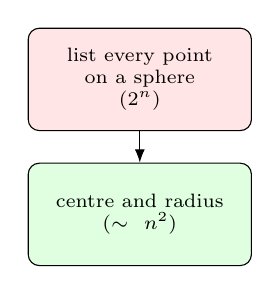
\begin{tikzpicture}[font=\scriptsize]
        \node[draw, fill=red!10, rounded corners, text width=2.6cm, align=center, minimum height=1.3cm]
          (a) {list every point\\ on a sphere\\ ($2^n$)};
        \node[draw, fill=green!12, rounded corners, text width=2.6cm, align=center, minimum height=1.3cm, below=4mm of a]
          (b) {centre and radius\\ ($\sim n^2$)};
        \draw[-{Latex}] (a) -- (b);
      \end{tikzpicture}
    \end{column}
  \end{columns}
  \vfill
  \alert{The catch.} No room for:
  \begin{itemize}
    \item non-Clifford gates ($T$, Toffoli)
    \item arbitrary superpositions
    \item mixed states
  \end{itemize}
\end{frame}

\begin{frame}{The alphabet (this is the whole trick)}
  \begin{columns}[c]
    \begin{column}{0.40\textwidth}
      \centering
      \begin{tabular}{cl}
        \toprule
        symbol & meaning \\
        \midrule
        $I$ & do nothing \\
        $X$ & flip the bit \\
        $Z$ & flip the sign \\
        $Y$ & both \\
        \bottomrule
      \end{tabular}
    \end{column}
    \begin{column}{0.56\textwidth}
      Each symbol is \textbf{2 bits} $(x,z)$ with one sign bit.
      \vspace{2mm}
      \begin{center}\large gate $=$ rewrite bits with XOR and AND\end{center}
      \vspace{1mm}
      No floating point, so it packs 64 qubits per machine word.
    \end{column}
  \end{columns}
\end{frame}

\begin{frame}{Why stabilizer simulators are everywhere}
  \alert{Plain idea:} random Clifford circuits mimic Haar-random ones, yet stay classically simulable.
  \vfill
  \begin{columns}[c]
    \begin{column}{0.46\textwidth}
      \centering
      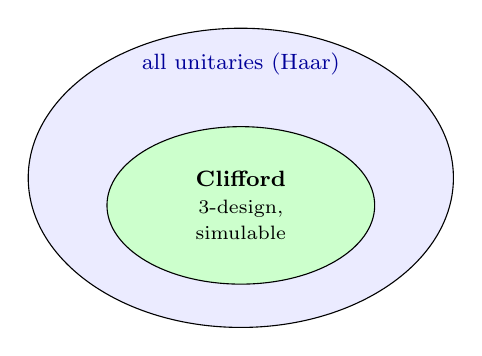
\begin{tikzpicture}[font=\footnotesize]
        \draw[fill=blue!8] (0,0) ellipse (2.7 and 1.9);
        \node[blue!60!black] at (0,1.45) {all unitaries (Haar)};
        \draw[fill=green!20] (0,-0.35) ellipse (1.7 and 1.0);
        \node[align=center] at (0,-0.35) {\textbf{Clifford}\\ \scriptsize 3-design,\\ \scriptsize simulable};
      \end{tikzpicture}
    \end{column}
    \begin{column}{0.5\textwidth}
      A \textbf{unitary 3-design} matches Haar-random unitaries up to the 3rd statistical moment.
      The Clifford group is one. So it stands in for ``random circuit'' in:
      \begin{itemize}
        \item randomized benchmarking
        \item classical shadows, tomography
        \item error correction (codes are Clifford)
      \end{itemize}
    \end{column}
  \end{columns}
\end{frame}

\begin{frame}{Two kinds of noise}
  \centering
  \begin{tabular}{lll}
    \toprule
     & \textbf{Pauli noise} & \textbf{Coherent / damping} \\
    \midrule
    what it is & random $X$, $Z$ flips & systematic tilt, energy loss \\
    stabilizer formalism & stays inside & \textbf{breaks it} \\
    stim & \checkmark & $\times$ \\
    qliff & \checkmark & \textbf{\checkmark} (quasiprobability) \\
    \bottomrule
  \end{tabular}
  \vfill
  \begin{center}\small
    qliff does the hard kind by a weighted-average method, nearly as cheap as the easy kind. \textbf{This is the differentiator.}
  \end{center}
\end{frame}

\begin{frame}{Why?}
  \alert{Plain idea:} noisy simulation at thousands of qubits, which a state-vector simulator cannot reach. Required for the Edge effects work
  \vfill
  \begin{columns}[c]
    \begin{column}{0.4\textwidth}
      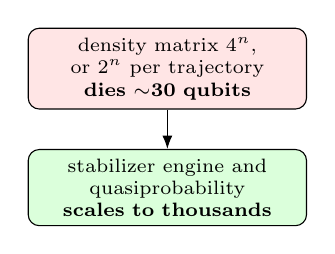
\begin{tikzpicture}[font=\scriptsize]
        \node[draw, fill=red!10, rounded corners, text width=3.3cm, align=center]
          (a) {density matrix $4^n$, or $2^n$ per trajectory \\ \textbf{dies $\sim$30 qubits}};
        \node[draw, fill=green!14, rounded corners, text width=3.3cm, align=center, below=5mm of a]
          (b) {stabilizer engine and quasiprobability \\ \textbf{scales to thousands}};
        \draw[-{Latex}] (a) -- (b);
      \end{tikzpicture}
    \end{column}
    \begin{column}{0.59\textwidth}
      \textbf{Myers, Teo, Mishra, Chai, Ng}\\
      \emph{Simulating general noise nearly as cheaply as Pauli noise}\\
      arXiv:2512.07304 (NUS)
      \vspace{2mm}
      \begin{itemize}
        \item any channel becomes signed stabilizer ops
        \item stratified importance sampling
      \end{itemize}
    \end{column}
  \end{columns}
\end{frame}

\begin{frame}{The two jobs, concretely}
  \begin{columns}[T]
    \begin{column}{0.5\textwidth}
      \textbf{Clean, Pauli (like stim)}
      \begin{itemize}
        \item bit-packed tableau, frame sampling
      \end{itemize}
      \vspace{1mm}
      {\small\texttt{Circuit().H(0).CX(0,1).M(0,1)}}
    \end{column}
    \begin{column}{0.5\textwidth}
      \textbf{Coherent (stim cannot)}
      \begin{itemize}
        \item $E=\sum_\mu q_\mu S_\mu$, signed weights
        \item importance-sample $\langle O\rangle$
      \end{itemize}
      \vspace{1mm}
      {\small\texttt{c.RZ(0,$\theta$).estimate("X")} $\approx \cos\theta$}
    \end{column}
  \end{columns}
  \vfill
  \begin{center}\small One engine: the noisy estimator runs many pure-Clifford trajectories and averages them.\end{center}
\end{frame}

% ======================================================================
\section{Bit packing}
% ======================================================================

\begin{frame}{The tableau (CHP)}
  $2n+1$ rows: $n$ destabilizers, $n$ stabilizers, $1$ scratch row.
  \vfill
  \begin{center}
  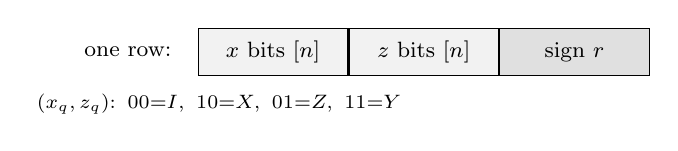
\begin{tikzpicture}[font=\footnotesize, node distance=0pt]
    \tikzset{cell/.style={draw, minimum width=1.9cm, minimum height=0.6cm}}
    \node[cell, fill=black!5] (x) {$x$ bits $[n]$};
    \node[cell, right=of x, fill=black!5] (z) {$z$ bits $[n]$};
    \node[cell, right=of z, fill=black!12] (r) {sign $r$};
    \node[left=6pt of x] {one row:};
    \node[below=3pt of x, text width=6cm, align=left]
      {\scriptsize $(x_q,z_q)$: $00{=}I,\ 10{=}X,\ 01{=}Z,\ 11{=}Y$};
  \end{tikzpicture}
  \end{center}
  \vfill
  \begin{center}\small
    $x,z$ are \code{Vec<u64>}, $W=\lceil n/64\rceil$ words per row. The scratch row is bookkeeping: it holds the running
    measurement product so the answer falls out in place.
  \end{center}
\end{frame}

\begin{frame}{Row-major: store the grid one row at a time}
  \begin{center}\small
    The tableau is a grid: one \textbf{row} per (de)stabilizer, one \textbf{column} per qubit. Memory is 1D, so we pick an order.
  \end{center}
  \vfill
  \begin{center}
  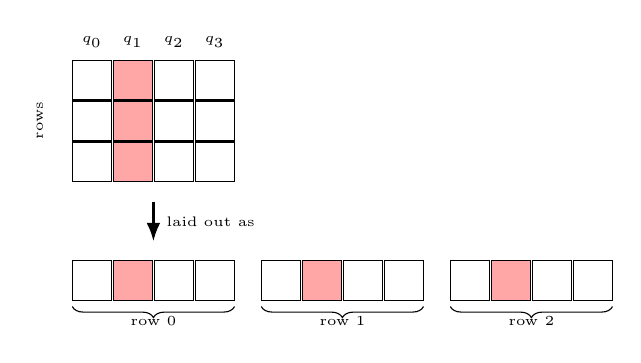
\begin{tikzpicture}[font=\scriptsize, cell/.style={draw, minimum size=0.5cm, inner sep=0pt}]
    % 2D grid: rows down, qubits across; highlight one qubit's column
    \foreach \r in {0,1,2} \foreach \c in {0,1,2,3}
      \node[cell] (g\r\c) at (\c*0.52,-\r*0.52) {};
    \foreach \r in {0,1,2} \node[cell, fill=red!35] at (0.52,-\r*0.52) {};
    \foreach \c in {0,1,2,3} \node[above=1pt, font=\tiny] at (g0\c.north) {$q_\c$};
    \node[rotate=90, anchor=south, font=\tiny] at (-0.5,-0.52) {rows};
    \draw[-{Latex}, thick] (0.78,-1.55) -- (0.78,-2.05) node[midway, right=1pt, font=\tiny] {laid out as};
    % 1D memory: row block after row block; the red qubit is now scattered
    \def\sy{-2.55}
    \foreach \r in {0,1,2} \foreach \c in {0,1,2,3} {
      \pgfmathsetmacro\xx{\r*2.4 + \c*0.52}
      \node[cell] at (\xx,\sy) {};
    }
    \foreach \r in {0,1,2} {
      \pgfmathsetmacro\xx{\r*2.4 + 0.52}
      \node[cell, fill=red!35] at (\xx,\sy) {};
    }
    \foreach \r in {0,1,2} {
      \pgfmathsetmacro\xa{\r*2.4 - 0.25}
      \pgfmathsetmacro\xb{\r*2.4 + 1.81}
      \draw[decorate, decoration={brace, mirror, amplitude=4pt}] (\xa,\sy-0.33) -- (\xb,\sy-0.33)
        node[midway, below, font=\tiny] {row \r};
    }
  \end{tikzpicture}
  \end{center}
  \vfill
  \begin{center}\small
    A \textcolor{red}{gate} hits one qubit across all rows (a column), so its cells are \textbf{strided}; a \textbf{measurement} combines whole rows, which sit \textbf{contiguous}.\\[2pt]
    \textbf{So row-major is the fast layout for measurement.} Gates fall off the \textbf{cache cliff} at large $n$ (Wall 1).
  \end{center}
\end{frame}

\begin{frame}{Column-major: store the grid one qubit-plane at a time}
  \begin{center}\small
    Same grid, swapped order: write each qubit's whole column before moving to the next.
  \end{center}
  \vfill
  \begin{center}
  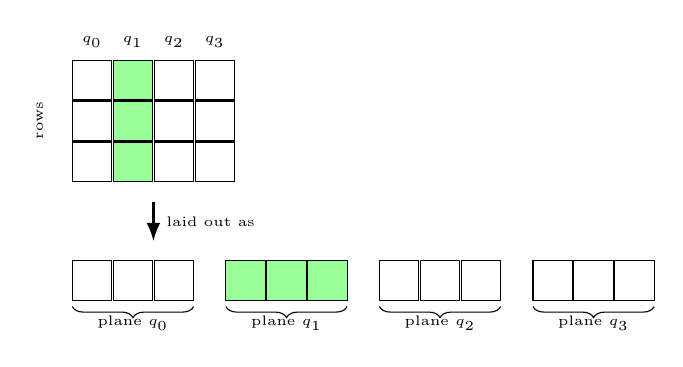
\begin{tikzpicture}[font=\scriptsize, cell/.style={draw, minimum size=0.5cm, inner sep=0pt}]
    \foreach \r in {0,1,2} \foreach \c in {0,1,2,3}
      \node[cell] (g\r\c) at (\c*0.52,-\r*0.52) {};
    \foreach \r in {0,1,2} \node[cell, fill=green!40] at (0.52,-\r*0.52) {};
    \foreach \c in {0,1,2,3} \node[above=1pt, font=\tiny] at (g0\c.north) {$q_\c$};
    \node[rotate=90, anchor=south, font=\tiny] at (-0.5,-0.52) {rows};
    \draw[-{Latex}, thick] (0.78,-1.55) -- (0.78,-2.05) node[midway, right=1pt, font=\tiny] {laid out as};
    % 1D memory: plane after plane; the green qubit is now one contiguous block
    \def\sy{-2.55}
    \foreach \c in {0,1,2,3} \foreach \r in {0,1,2} {
      \pgfmathsetmacro\xx{\c*1.95 + \r*0.52}
      \node[cell] at (\xx,\sy) {};
    }
    \foreach \r in {0,1,2} {
      \pgfmathsetmacro\xx{1.95 + \r*0.52}
      \node[cell, fill=green!40] at (\xx,\sy) {};
    }
    \foreach \c in {0,1,2,3} {
      \pgfmathsetmacro\xa{\c*1.95 - 0.25}
      \pgfmathsetmacro\xb{\c*1.95 + 1.29}
      \draw[decorate, decoration={brace, mirror, amplitude=4pt}] (\xa,\sy-0.33) -- (\xb,\sy-0.33)
        node[midway, below, font=\tiny] {plane $q_\c$};
    }
  \end{tikzpicture}
  \end{center}
  \vfill
  \begin{center}\small
    Now a \textcolor{green!50!black}{gate} sweeps one qubit-plane, all \textbf{contiguous} (cache cliff gone); a \textbf{measurement} must hop plane to plane, so it is \textbf{strided}.\\[2pt]
    \textbf{So column-major is the fast layout for gates.} We keep both layouts and transpose at the gate/measure boundary.
  \end{center}
\end{frame}

% ======================================================================
\section{Optimizations}
% ======================================================================

\begin{frame}{The map: two loops, two walls}
  \begin{columns}[T]
    \begin{column}{0.5\textwidth}
      \centering\textbf{Inner loop: the tableau}\\
      {\scriptsize cost of one Clifford gate or measurement}
      \vspace{2mm}
      \begin{itemize}
        \item faster measurement (combine rows wordwise)
        \item one-pass \code{CZ}
        \item \alert{Wall 1}: gates at large $n$, fixed by column-major
        \item batch across the Python/Rust border
      \end{itemize}
    \end{column}
    \begin{column}{0.5\textwidth}
      \centering\textbf{Outer loop: noisy sampling}\\
      {\scriptsize many shots of one noisy circuit}
      \vspace{2mm}
      \begin{itemize}
        \item \alert{Wall 2}: re-running per shot, fixed by Pauli frames
        \item skip the shots that do not fault
        \item zero-copy \code{numpy} output
        \item run on all CPU cores
      \end{itemize}
    \end{column}
  \end{columns}
  \vfill
  \begin{center}\small Then the payoff: the coherent-noise estimator, the thing stim cannot do, moved into parallel Rust.\end{center}
\end{frame}

\begin{frame}{Noisy sampling: the wins stack up ($n=1024$)}
  \centering
  \begin{tikzpicture}
  \begin{axis}[
      ymode=log, width=0.9\textwidth, height=0.62\textheight,
      ybar, bar width=15pt,
      symbolic x coords={per-shot, layout, batch, frames, skip-rare, numpy, ref-run},
      xtick=data, x tick label style={rotate=25, anchor=east, font=\scriptsize},
      ylabel={ms / shot (log)}, ymin=0.0008, ymax=80,
      grid=both, major grid style={black!10},
      legend pos=north east, legend cell align=left,
    ]
    \addplot[fill=blue!55] coordinates {
      (per-shot,41) (layout,13) (batch,5.1) (frames,0.020) (skip-rare,0.012) (numpy,0.0069) (ref-run,0.00134) };
    \addplot[red, dashed, very thick, no markers, sharp plot] coordinates {(per-shot,0.00357) (ref-run,0.00357)};
    \addlegendentry{qliff}
    \addlegendentry{stim clean}
  \end{axis}
  \end{tikzpicture}
  \par\footnotesize Each bar applies one more technique. From 41 to 0.0013 ms/shot, about \textbf{30000$\times$}, dropping below stim's clean sampler.
\end{frame}

\begin{frame}{Opt 1: combine rows 64 bits at a time}
  \alert{Was slow:} a measurement combines two tableau rows qubit-by-qubit, a serial $O(n)$ loop.
  \vfill
  \begin{center}\large
    per-qubit loop, $O(n)$ \quad$\Longrightarrow$\quad whole words at once (bitwise ops and a popcount), $O(n/64)$
  \end{center}
  \vfill
  \begin{center}\large Measurement flips from \textbf{$2.6\times$ slower} than stim to \textbf{$2\times$ faster}.\end{center}
\end{frame}

\begin{frame}{Opt 2: one-pass \code{CZ}}
  \alert{Was slow:} \code{CZ} was built from \code{H, CX, H}, three full sweeps over a qubit-plane.
  \vfill
  \begin{center}\large \code{H, CX, H} (3 sweeps) $\;\Longrightarrow\;$ one symmetric update (1 sweep)\end{center}
  \vfill
  \begin{center}\large \textbf{$2\times$ faster \code{CZ}}; surface codes are \code{CZ}-heavy. Verified over 400 circuits.\end{center}
\end{frame}

\begin{frame}{Opt 3: Wall 1, the cache cliff (column-major)}
  \alert{Was slow:} in row-major a gate strides across rows; past $n\approx512$ every read misses cache.
  \vfill
  \begin{center}
  \begin{tabular}{lr}
    \toprule
    gate path at $n=1024$ & vs stim \\
    \midrule
    row-major (strided reads) & $\sim 11\times$ slower \\
    \textbf{column-major (contiguous planes)} & \textbf{$1.2\times$ faster} \\
    \bottomrule
  \end{tabular}
  \end{center}
  \vfill
  \begin{center}\small Contiguous planes erase the stride: raw tableau $\sim$10.7 M/s, about $4\times$ stim at $n=1024$.\end{center}
\end{frame}

\begin{frame}{Opt 4: batch across the Python/Rust border}
  \alert{Was slow:} each gate was its own call from Python into Rust; at millions of gates/s that border dominates.
  \vfill
  \begin{center}\large one call per gate $\;\Longrightarrow\;$ one call per block of gates\end{center}
  \vfill
  \begin{itemize}
    \item \code{Circuit.run} batches to $\sim$20 M/s at $n=1024$, about $8\times$ stim.
    \item the whole noisy Monte-Carlo loop now runs inside Rust.
    \item custom Python noise channels still work, on a slower fallback path.
  \end{itemize}
\end{frame}

\begin{frame}{Opt 5: Wall 2, the Pauli-frame sampler}
  \alert{Was slow:} noisy sampling re-ran the entire circuit from scratch, once per shot.
  \vfill
  \begin{center}
  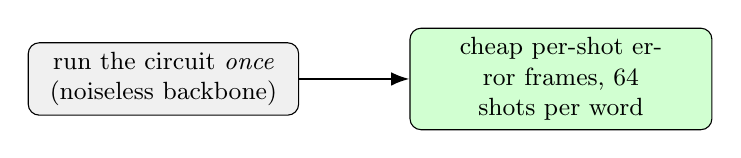
\begin{tikzpicture}[font=\small, node distance=14mm]
    \node[draw, rounded corners, fill=black!6, text width=3.2cm, align=center] (ref) {run the circuit \emph{once} (noiseless backbone)};
    \node[draw, rounded corners, fill=green!18, right=of ref, text width=3.6cm, align=center] (fr) {cheap per-shot error frames, 64 shots per word};
    \draw[-{Latex}, thick] (ref) -- (fr);
  \end{tikzpicture}
  \end{center}
  \vfill
  \begin{center}\large $41$ ms/shot $\;\Longrightarrow\;$ \textbf{0.020 ms/shot}, about $5\times$ stim clean.\end{center}
\end{frame}

\begin{frame}{Opt 5 (cont.): when frames do not apply}
  \alert{The catch:} frames assume the noiseless run fixes each measurement, with noise only flipping it.
  \vfill
  \begin{center}
  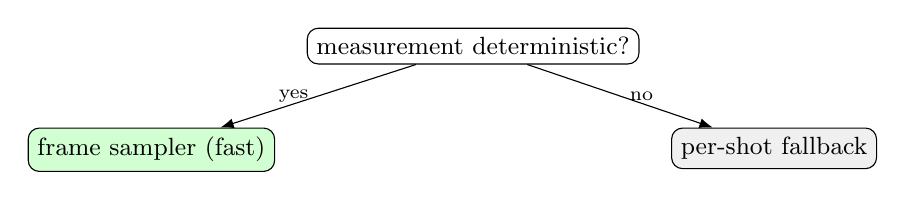
\begin{tikzpicture}[font=\small, node distance=10mm]
    \node[draw, rounded corners] (q) {measurement deterministic?};
    \node[draw, rounded corners, fill=green!18, below left=8mm and 4mm of q] (y) {frame sampler (fast)};
    \node[draw, rounded corners, fill=black!6, below right=8mm and 4mm of q] (n) {per-shot fallback};
    \draw[-{Latex}] (q) -- node[left, font=\scriptsize]{yes} (y);
    \draw[-{Latex}] (q) -- node[right, font=\scriptsize]{no} (n);
  \end{tikzpicture}
  \end{center}
  \vfill
  \begin{center}\small A random measurement cannot ride along in a frame, so it routes to the per-shot path. QEC syndromes are deterministic, so they stay fast.\end{center}
\end{frame}

\begin{frame}{Opt 6: skip the shots that do not fault}
  \alert{Was slow:} we flipped a coin for every (noise location, shot) pair, even though faults are rare.
  \vfill
  \begin{center}\large draw the gap to the next faulting shot, then jump straight there\end{center}
  \vfill
  \begin{center}\large touch only $\sim\phi\cdot\text{shots}$, a $\sim 1/\phi$ win. At $\phi=10^{-3}$: $0.020 \to$ \textbf{0.012 ms/shot}.\end{center}
\end{frame}

\begin{frame}{Opt 7: hand back raw bytes, not Python ints}
  \alert{Was slow:} each measured bit was boxed into a Python integer, millions of allocations per sample.
  \vfill
  \begin{center}\large
    $\sim$5M boxed Python ints \quad$\Longrightarrow$\quad one flat byte buffer viewed as a \code{numpy} array (zero copy)
  \end{center}
  \vfill
  \begin{center}\large Killed $\sim$40\% of per-shot time: $0.012 \to$ \textbf{0.0069 ms/shot}.\end{center}
\end{frame}

\begin{frame}{Opt 8: use every CPU core}
  \alert{Was slow:} the sampler ran on a single core while the rest sat idle.
  \vfill
  \begin{center}
  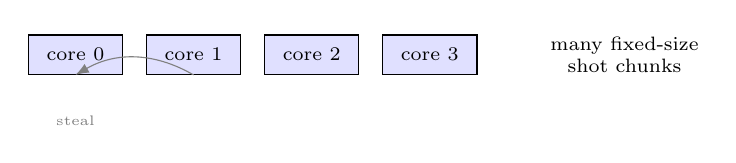
\begin{tikzpicture}[font=\scriptsize, node distance=3mm]
    \foreach \i/\x in {0/0,1/1.5,2/3,3/4.5} {
      \node[draw, fill=blue!12, minimum width=1.2cm, minimum height=0.5cm] (core\i) at (\x,0) {core \i};
    }
    \node[align=center, right=8mm of core3] {many fixed-size\\ shot chunks};
    \draw[-{Latex}, gray] (core1.south) to[bend right] (core0.south);
    \node[gray, font=\tiny, below=4mm of core0] {steal};
  \end{tikzpicture}
  \end{center}
  \vfill
  \begin{center}\large Idle cores steal chunks from busy ones. \textbf{2.6$\times$} on 8 cores at 200k shots; fixed chunks keep results reproducible.\end{center}
\end{frame}

\begin{frame}{Opt 9: the hard-noise estimator, in parallel Rust}
  \alert{The payoff:} coherent and general noise (which stim cannot do) ran as a slow Python loop.
  \vfill
  \begin{center}\Large coherent / general $\langle O\rangle$:\quad Python loop $\;\Longrightarrow\;$ multicore Rust\end{center}
  \vfill
  \begin{center}\Large \textbf{229$\times$ faster} (5793 ms $\to$ 25 ms), validated unbiased.\end{center}
  \par\footnotesize $R_Z(\theta) \to \langle X\rangle = \cos\theta$;\quad amplitude damping on $|1\rangle \to \langle Z\rangle = 2p-1$.
\end{frame}


\begin{frame}{1 qubit: the X gate}
  State $|0\rangle$, stabilizer $+Z$. Rule: $r \mathrel{\oplus}= z$.
  \vfill
  \begin{center}\large
  \begin{tabular}{lcccl}
    \toprule
     & $x$ & $z$ & $r$ & Pauli \\
    \midrule
    before & 0 & 1 & 0 & $+Z$, stabilizes $|0\rangle$ \\
    after  & 0 & 1 & \textbf{1} & $-Z$, stabilizes $|1\rangle$ \\
    \bottomrule
  \end{tabular}
  \end{center}
  \vfill
  \begin{center}\small $z=1$, so the sign flips: $X|0\rangle=|1\rangle$. $X$ flips any row with a $Z$-component.\end{center}
\end{frame}

\begin{frame}{1 qubit: the H gate}
  State $|0\rangle$, stabilizer $+Z$. Rule: swap $x\!\leftrightarrow\!z$, then $r \mathrel{\oplus}= x\,z$.
  \vfill
  \begin{center}\large
  \begin{tabular}{lcccl}
    \toprule
     & $x$ & $z$ & $r$ & Pauli \\
    \midrule
    before & 0 & 1 & 0 & $+Z$, stabilizes $|0\rangle$ \\
    after  & \textbf{1} & \textbf{0} & 0 & $+X$, stabilizes $|{+}\rangle$ \\
    \bottomrule
  \end{tabular}
  \end{center}
  \vfill
  \begin{center}\small $x\,z=0$, so no sign flip; the swap turns $Z$ into $X$: $H|0\rangle=|{+}\rangle$.\end{center}
\end{frame}

\begin{frame}{2 qubits: X on one qubit}
  State $|00\rangle$, generators $+ZI$ and $+IZ$. Apply $X$ on qubit 0 ($r \mathrel{\oplus}= z_{q0}$).
  \vfill
  \begin{center}\large
  \begin{tabular}{lcccl}
    \toprule
    generator & $x\,(q_0q_1)$ & $z\,(q_0q_1)$ & $r$ & Pauli \\
    \midrule
    $g_1$ before & 00 & 10 & 0 & $+ZI$ \\
    $g_1$ after  & 00 & 10 & \textbf{1} & $-ZI$ \\[2pt]
    $g_2$ & 00 & 01 & 0 & $+IZ$, untouched \\
    \bottomrule
  \end{tabular}
  \end{center}
  \vfill
  \begin{center}\small Only $g_1$ has $z_{q0}=1$, so only its sign flips: $|00\rangle \to |10\rangle$.\end{center}
\end{frame}

\begin{frame}{2 qubits: CX builds a Bell pair}
  $|00\rangle \xrightarrow{\,H(0)\,}\ \xrightarrow{\,CX(0\to1)\,}$ Bell state.
  \vfill
  \begin{center}\large
  \begin{tabular}{lll}
    \toprule
    after $H(0)$ & apply CX$(0\!\to\!1)$ & result \\
    \midrule
    $+XI$ & $x_1 \mathrel{\oplus}= x_0$: $XI \to XX$ & $+XX$ \\
    $+IZ$ & $z_0 \mathrel{\oplus}= z_1$: $IZ \to ZZ$ & $+ZZ$ \\
    \bottomrule
  \end{tabular}
  \end{center}
  \vfill
  \begin{center}\small
    $\{+XX,+ZZ\}$ is the Bell state. Matches \code{Simulator(2).H(0).CX(0,1).canon()} $=$ \code{['+XX','+ZZ']}.
  \end{center}
\end{frame}


\section{Benchmarks}
% ===============================================

\begin{frame}{Gate throughput (ns per gate), versus stim}
  \centering
  \begin{tikzpicture}
  \begin{loglogaxis}[
      width=0.82\textwidth, height=0.66\textheight,
      xlabel={qubits $n$}, ylabel={ns per gate},
      log basis x=2, xtick={64,256,1024,4096,16384,65536},
      xticklabels={64,256,1k,4k,16k,64k},
      legend pos=north west, legend cell align=left,
      error bars/y dir=both, error bars/y explicit,
      grid=both, major grid style={black!10},
    ]
    \addplot+[mark=*] coordinates {
      (64,324.028) +- (0,3.934) (256,334.991) +- (0,1.919) (1024,360.190) +- (0,0.525)
      (4096,416.276) +- (0,6.964) (16384,974.685) +- (0,54.632) (65536,15300.6) +- (0,1374.66) };
    \addlegendentry{qliff}
    \addplot+[mark=square*] coordinates {
      (64,406.233) +- (0,4.998) (256,419.115) +- (0,3.719) (1024,459.686) +- (0,0.555)
      (4096,548.108) +- (0,8.407) (16384,1312.50) +- (0,61.281) (65536,22790.5) +- (0,1600.55) };
    \addlegendentry{stim 1.16}
  \end{loglogaxis}
  \end{tikzpicture}
  \par\footnotesize No crossover: qliff leads at every size and the gap widens, \textbf{1.5$\times$} at $n=65536$. (Single-gate dispatch, mix 34\% H / 33\% S / 33\% CX.)
\end{frame}

\begin{frame}{Measurement throughput (ns per measurement)}
  \centering
  \begin{tikzpicture}
  \begin{loglogaxis}[
      width=0.82\textwidth, height=0.66\textheight,
      xlabel={qubits $n$}, ylabel={ns per measurement},
      log basis x=2, xtick={16,32,64,128,256,512,1024},
      xticklabels={16,32,64,128,256,512,1024},
      legend pos=north west, legend cell align=left,
      error bars/y dir=both, error bars/y explicit,
      grid=both, major grid style={black!10},
    ]
    \addplot+[mark=*] coordinates {
      (16,134.974) +- (0,7.258) (32,150.19) +- (0,2.62) (64,196.932) +- (0,4.588)
      (128,306.94) +- (0,2.118) (256,503.841) +- (0,6.317) (512,801.555) +- (0,4.595)
      (1024,1657.94) +- (0,19.44) };
    \addlegendentry{qliff}
    \addplot+[mark=square*] coordinates {
      (16,262.299) +- (0,182.6) (32,191.663) +- (0,2.546) (64,185.504) +- (0,0.7488)
      (128,253.887) +- (0,1.356) (256,505.505) +- (0,8.932) (512,1678.78) +- (0,6.884)
      (1024,4194.35) +- (0,22.38) };
    \addlegendentry{stim 1.16}
  \end{loglogaxis}
  \end{tikzpicture}
  \par\footnotesize Crossover near $n=64$ to $256$; at scale qliff pulls ahead, \textbf{2.5$\times$} at $n=1024$.
\end{frame}

\begin{frame}{Noisy sampling (ms per shot), versus stim clean}
  \centering
  \begin{tikzpicture}
  \begin{loglogaxis}[
      width=0.82\textwidth, height=0.64\textheight,
      xlabel={qubits $n$}, ylabel={ms per shot},
      log basis x=2, xtick={16,32,64,128,256,512,1024},
      xticklabels={16,32,64,128,256,512,1024},
      legend pos=north west, legend cell align=left,
      error bars/y dir=both, error bars/y explicit,
      grid=both, major grid style={black!10},
    ]
    \addplot+[mark=*] coordinates {
      (16,2.44071e-05) +- (0,1.405e-05) (32,3.10202e-05) +- (0,1.04e-06) (64,7.01792e-05) +- (0,1.676e-05)
      (128,0.000120684) +- (0,4.186e-06) (256,0.000260307) +- (0,2.372e-05) (512,0.000546476) +- (0,4.179e-05)
      (1024,0.00132492) +- (0,9.788e-05) };
    \addlegendentry{qliff noisy}
    \addplot+[mark=square*] coordinates {
      (16,6.49107e-05) +- (0,6.015e-05) (32,6.02631e-05) +- (0,7.348e-07) (64,0.000114429) +- (0,9.79e-07)
      (128,0.000247043) +- (0,4.925e-06) (256,0.000540785) +- (0,3.296e-05) (512,0.00167698) +- (0,3.664e-05)
      (1024,0.0040025) +- (0,7.602e-05) };
    \addlegendentry{stim noisy}
    \addplot+[mark=triangle*] coordinates {
      (16,3.23036e-05) +- (0,6.651e-07) (32,4.76711e-05) +- (0,3.494e-07) (64,8.74536e-05) +- (0,1.147e-06)
      (128,0.000189542) +- (0,2.386e-06) (256,0.000421127) +- (0,2.814e-05) (512,0.00146467) +- (0,4.57e-05)
      (1024,0.00356751) +- (0,9.398e-05) };
    \addlegendentry{stim clean}
  \end{loglogaxis}
  \end{tikzpicture}
  \par\footnotesize qliff noisy beats stim clean at every size, \textbf{2.7$\times$} at $n=1024$. (DEPOLARIZE1, $p=10^{-3}$.)
\end{frame}

% ======================================================================
\section{Features}
% ======================================================================

\begin{frame}{Feature comparison}
  \centering
  \small
  \begin{tabular}{lcc}
    \toprule
    capability & qliff & stim \\
    \midrule
    Clifford tableau, mid-circuit measure, reset, feedback & \checkmark & \checkmark \\
    Bit-packed frame sampling, multicore & \checkmark & \checkmark \\
    Pauli noise (depolarize, X/Z error, Pauli channel) & \checkmark & \checkmark \\
    Detectors, observables, DEM export for decoders & \checkmark & \checkmark \\
    \textbf{Coherent and amplitude-damping noise} & \textbf{\checkmark} & $\times$ \\
    \textbf{Quasiprobability importance estimator} & \textbf{\checkmark} & $\times$ \\
    \textbf{Python-first custom channels, no recompile} & \textbf{\checkmark} & $\times$ \\
    Circuit file format, diagrams, large gate zoo & $\times$ & \checkmark \\
    Tableau, PauliString, Flow algebra objects & $\times$ & \checkmark \\
    Many built-in code families, mature ecosystem & 2 codes & \checkmark \\
    \bottomrule
  \end{tabular}
\end{frame}

\end{document}
